%%%%%%%%%%%%%%%%%%%%%%%%%%%%%%%%%%%%%%%%%%%%%%%%%%%%%%%%
%                       Assignment 2                   %
%                                                      %
% Author: Michael P. J. Camilleri					   %
%                                                      %
% Based on the Cleese Assignment Template for Students %
% from http://www.LaTeXTemplates.com.				   %
%                                                      %
% Original Author: Vel (vel@LaTeXTemplates.com)		   %
%													   %
% License:											   %
% CC BY-NC-SA 3.0 									   %
% (http://creativecommons.org/licenses/by-nc-sa/3.0/)  %
% 													   %
%%%%%%%%%%%%%%%%%%%%%%%%%%%%%%%%%%%%%%%%%%%%%%%%%%%%%%%%

%--------------------------------------------------------
%   IMPORTANT: Do not touch anything in this part
\documentclass[12pt]{article}
%%%%%%%%%%%%%%%%%%%%%%%%%%%%%%%%%%%%%%%%%
% Cleese Assignment
% Structure Specification File
% Version 1.0 (27/5/2018)
%
% This template originates from:
% http://www.LaTeXTemplates.com
%
% Author:
% Vel (vel@LaTeXTemplates.com)
%
% License:
% CC BY-NC-SA 3.0 (http://creativecommons.org/licenses/by-nc-sa/3.0/)
% 
%%%%%%%%%%%%%%%%%%%%%%%%%%%%%%%%%%%%%%%%%

%----------------------------------------------------------------------------------------
%	PACKAGES AND OTHER DOCUMENT CONFIGURATIONS
%----------------------------------------------------------------------------------------

\usepackage{lastpage} % Required to determine the last page number for the footer
\usepackage{graphicx} % Required to insert images
\setlength\parindent{0pt} % Removes all indentation from paragraphs
\usepackage[most]{tcolorbox} % Required for boxes that split across pages
\usepackage{booktabs} % Required for better horizontal rules in tables
\usepackage{listings} % Required for insertion of code
\usepackage{etoolbox} % Required for if statements
\usepackage{geometry} % Required for adjusting page dimensions and margins
\usepackage[utf8]{inputenc} % Required for inputting international characters
\usepackage[T1]{fontenc} % Output font encoding for international characters
\usepackage{fancyhdr} % Required for customising headers and footers
\usepackage{xspace}
\usepackage{booktabs}
\usepackage[colorlinks]{hyperref}
\usepackage{etoolbox}

\newcommand{\ie}{i.e.\@\xspace}
\newcommand{\eg}{e.g.\@\xspace}
\newcommand{\notemark}[1]{\textcolor{blue}{N.B.\ \emph{#1}}}
\newcommand{\noteself}[1]{\textcolor{red}{Thought: \emph{#1}}}
\newcommand{\note}[1]{\emph{\textbf{N.B.}\@\xspace#1}}
\newcommand{\hint}[1]{\emph{Hint: #1}}
\newcommand{\half}{$\frac{1}{2}$ }

\newbool{clearnext}		%Running Counter to see if clearing the page or not in the next subquestion.
\newbool{clearon}		%Parameter for specifying whether we will be clearing or not.
\newbool{authoron}		%Parameter to specify whether to show author or not

%----------------------------------------------------------------------------------------
%	Standard Template
%----------------------------------------------------------------------------------------
\geometry{
	paper=a4paper, % Change to letterpaper for US letter
	top=3cm, % Top margin
	bottom=3cm, % Bottom margin
	left=2.5cm, % Left margin
	right=2.5cm, % Right margin
	headheight=14pt, % Header height
	footskip=1.4cm, % Space from the bottom margin to the baseline of the footer
	headsep=1.2cm, % Space from the top margin to the baseline of the header
	%showframe, % Uncomment to show how the type block is set on the page
}
\pagestyle{fancy} % Enable custom headers and footers

%----------------------------------------------------------------------------------------
%	My Changes
%----------------------------------------------------------------------------------------
\lhead{\small\assignmentClass}
\chead{}
\ifbool{authoron}{\rhead{\small{\assignmentAuthorName}}}{\rhead{}}

\lfoot{} % Left footer
\cfoot{} % Centre footer
\rfoot{\small Page\ \thepage\ of\ \pageref{LastPage}} % Right footer

\renewcommand\headrulewidth{0.5pt} % Thickness of the header rule

%----------------------------------------------------------------------------------------
%	MODIFY SECTION STYLES
%----------------------------------------------------------------------------------------

\usepackage{titlesec} % Required for modifying sections

%------------------------------------------------
% Section

\titleformat
{\section} % Section type being modified
[block] % Shape type, can be: hang, block, display, runin, leftmargin, rightmargin, drop, wrap, frame
{\Large\bfseries} % Format of the whole section
{\assignmentQuestionName~\thesection} % Format of the section label
{6pt} % Space between the title and label
{} % Code before the label

\titlespacing{\section}{0pt}{0.5\baselineskip}{0.5\baselineskip} % Spacing around section titles, the order is: left, before and after

%------------------------------------------------
% Subsection

\titleformat
{\subsection} % Section type being modified
[block] % Shape type, can be: hang, block, display, runin, leftmargin, rightmargin, drop, wrap, frame
{} % Format of the whole section
{[\arabic{section}.\arabic{subsection}]} % Format of the section label (\alph{subsection})
{4pt} % Space between the title and label
{} % Code before the label

\titlespacing{\subsection}{0pt}{0.5\baselineskip}{0.5\baselineskip} % Spacing around section titles, the order is: left, before and after

\renewcommand\thesubsection{(\arabic{subsection})}

%----------------------------------------------------------------------------------------
%	CUSTOM QUESTION COMMANDS/ENVIRONMENTS
%----------------------------------------------------------------------------------------

% Environment to be used for each question in the assignment
\newenvironment{question}[1]{
	\ifbool{clearon}{\clearpage}{}
	\global\setbool{clearnext}{false}
	\vspace{0.5\baselineskip} % Whitespace before the question
	\section{: #1}
	\lfoot{\small\itshape\assignmentQuestionName~\thesection~continued on next page\ldots} % Set the left footer to state the question continues on the next page, this is reset to nothing if it doesn't (below)
}{
	\lfoot{} % Reset the left footer to nothing if the current question does not continue on the next page
}

%------------------------------------------------

% Environment for inter-subquestion texts (no arguments)
\newenvironment{interquestiontext}{
	\ifbool{clearon}{\ifbool{clearnext}{\clearpage}{}}{}
	\global\setbool{clearnext}{false}
}{
}

%------------------------------------------------


%------------------------------------------------

% Environment for subquestions, takes 1 argument - the name of the section
\newenvironment{subquestion}[1]{
	\ifbool{clearon}{\ifbool{clearnext}{\clearpage}{}}{}
	\global\setbool{clearnext}{true}
	\subsection{#1}
}{
}

%------------------------------------------------

% Command to print a question sentence
\newcommand{\questiontext}[1]{
	\textbf{#1}
	\vspace{0.5\baselineskip} % Whitespace afterwards
	\global\setbool{clearnext}{false}
}

%------------------------------------------------
% Command to print a  Marking Scheme box.
\newcommand{\marking}[1]{
	\begin{tcolorbox}[colback=green!5!white,enhanced]
		\textbf{Marking Scheme:}#1
	\end{tcolorbox}
}

%------------------------------------------------

% Command to print a box that breaks across pages with the space for a student to answer
\newcommand{\model}[1]{
	\begin{tcolorbox}[enhanced]
		\textbf{Model Answer}:#1
	\end{tcolorbox}
}

\newcommand{\answerbox}[2]{
	\begin{tcolorbox}[enhanced, height=#1]
		#2
	\end{tcolorbox}
}

%------------------------------------------------

% Command to print an assignment section title to split an assignment into major parts
\newcommand{\assignmentSection}[1]{
	{
		\centering % Centre the section title
		\vspace{2\baselineskip} % Whitespace before the entire section title
		
		\rule{0.8\textwidth}{0.5pt} % Horizontal rule
		
		\vspace{0.75\baselineskip} % Whitespace before the section title
		{\LARGE \MakeUppercase{#1}} % Section title, forced to be uppercase
		
		\rule{0.8\textwidth}{0.5pt} % Horizontal rule
		
		\vspace{\baselineskip} % Whitespace after the entire section title
	}
}

%----------------------------------------------------------------------------------------
%	TITLE PAGE
%----------------------------------------------------------------------------------------

\title{
	\thispagestyle{empty} 		% Suppress headers and footers
	\vspace{0.01\textheight} 	% Whitespace before the title
	\textbf{\assignmentClass:\\ \assignmentTitle}\\[4pt]
	\ifbool{authoron}{\assignmentAuthorName}{
	\ifdef{\assignmentDueDate}{{\small Due\ on\ \assignmentDueDate}\\}{}
	{\large \textit{\assignmentWarning}}
	\vspace{0.01\textheight}} % Whitespace before the author name
}

\ifbool{authoron}{\author{Student: \textbf{\assignmentAuthorName}}}{}
\date{} % Don't use the default title page date field





% Options for Formatting Output

\global\setbool{clearon}{true} %
\global\setbool{authoron}{true} %



\newcommand{\assignmentQuestionName}{Question}
\newcommand{\assignmentTitle}{Assignment\ \#2}

\newcommand{\assignmentClass}{IAML -- INFR10069 (LEVEL 10)}

\newcommand{\assignmentWarning}{NO LATE SUBMISSIONS} % 
\newcommand{\assignmentDueDate}{Friday,\ November\ 15,\ 2019 @ 16:00}
%--------------------------------------------------------

%--------------------------------------------------------
%   IMPORTANT: Specify your Student ID below [You will need to uncomment the line, else compilation will fail]. Make sure to specify your student ID correctly, otherwise we may not be able to identify your work and you will be marked as missing.
\newcommand{\assignmentAuthorName}{s1701688}
%--------------------------------------------------------

\begin{document}
\maketitle
\thispagestyle{empty}



%%%%%%%%%%%%%%%%%%%%%%%%%%%%%%%%%%%%%%%%%%%%%%%%%%%%%%%%%%%%%%%%%%%%%%%%%%%%%%
%============================================================================%
%%%%%%%%%%%%%%%%%%%%%%%%%%%%%%%%%%%%%%%%%%%%%%%%%%%%%%%%%%%%%%%%%%%%%%%%%%%%%%


\assignmentSection{Part A: 20-NewsGroups [60 Points]}




\begin{question}{(10 points) Exploratory Analysis}

\questiontext{We will begin by exploring the Dataset to get some insight about it.}



\begin{subquestion}{(5 points) Focusing first on the training set, summarise the key features/observations in the data: focus on the dimensionality, data ranges, feature and class distribution and report anything out of the ordinary. What are the typical values of the features like?}


\answerbox{12em}{
Set has 5648 entries and 1000 attributes, with data that ranges from 0 to 1. All attributes are non-null and of type float64; and their mean values are quite low, although they seem greater than the median. Values for all percentiles is 0. By comparing the 75th percentile against the max value for each attribute, we could say that there are outliers in the dataset. Distribution of the classes is quite balanced, except for class 7, which has around 1/3 less instances than the others. Classes 0-1 (comp), 2-3 (rec), 4-5 (sci), 6-7 (religion) are closely related. There are only 110 unique values in our dataset, and it seems that there is only one value count for all the values except for 0. In fact, 5539 of our instances take value 0 in our dataset.
}



\end{subquestion}


\begin{subquestion}{(3 points) Looking now at the Testing set, how does it compare with the Training Set (in terms of sizes and feature-distributions) and what could be the repercussions of this?}


\answerbox{10em}{
There are less instances than training set (1883) and number of attributes remains the same. All values are non-null of type float64. There are 32 unique values (32/1883=0.017). The proportion of unique values is slightly lower than the one we have for our training dataset (110/5648=0.019), which is expected since we have less entries. Entries in testing are different to those in training, which is preferable to determine if the model generalises well. Like in the training dataset, there are less instances labeled 7 compared to the other classes.
}



\end{subquestion}

\begin{subquestion}{(2 points) Why do you think it is useful to consider TF-IDF weights as opposed to just the frequency of times a word appears in a document as a feature?}



\answerbox{10em}{
TF-IDF balances out the frequency of words by how often they appear across all documents; it reflects how relevant a word in a document is. It might be the case that a word is generally frequent, like 'the', but are not relevant nor meaningful. TF-IDF reduces the weight of these common meaningless words and gives higher weight to uncommon words in a document. If we used the number of times a word appears in a document, then we would get that extremely frequent words dominate in some documents, even if they do not provide any useful information to our model.
}



\end{subquestion}



\end{question}


%============================================================================%

\begin{question}{\label{Q_UNSUP_LEARN}(24 points) Unsupervised Learning}

\questiontext{We will now explore the documents in some detail by way of clustering.}



\begin{subquestion}{(2 points) The K-Means algorithm is non-deterministic. Explain why this is, and how the final model is selected in the SKLearn implementation of \href{https://scikit-learn.org/stable/modules/clustering.html}{KMeans}.}



\answerbox{8em}{
Since the initial centroids are randomly selected, on different executions of the algorithm, different outputs are obtained for the same dataset; which makes results hard to compare. The SKLearn implementation of k-means stops when the difference between previous and new centroids is less than a specific threshold. The algorithm runs until the centroids of the clusters do not change significantly. The final model is the one obtained when we stop after reaching the threshold.
}



\end{subquestion}


\begin{subquestion}{(1 point) One of the parameters we need to specify when using k-means is the number of clusters. What is a reasonable number for this problem and why?}



\answerbox{5em}{
By using the number of distinct classes we have in the dataset (8) as the number of clusters for k-means, we group the instances into 8 different clusters (each assigned to one label) and will obtain the label that corresponds to each datapoint.
}



\end{subquestion}


\begin{subquestion}{(5 points) We will use the Adjusted Mutual Information (AMI) \ie \href{https://scikit-learn.org/stable/modules/clustering.html\#mutual-info-score}{\texttt{adjusted\_mutual\\\_info\_score}} between the clusters and the true (known) labels to quantify the performance of the clustering. Give an expression for the MI in terms of entropy. In short, describe what the MI measures about two variables, why this is applicable here and why it might be difficult to use in practice. \hint{MI is sometimes referred to as Information Gain: note that you are asked only about the standard way we defined MI and not the AMI which is adjusted for the size of the domain and for chance agreement.}}



\answerbox{16em}{
MI in terms of entropy is MI(U,V) = H(U) + H(V) - H(U,V). It measures how accurate the clustering's label predictions are, compared to the actual true labels, i.e., how related to variables are to each other. It provides a general measure based on the joint probabilities of two variables assuming no underlying relationship (like linearity). MI is capable of identifying more information about the relationship of two variables than correlation can. It is applicable here because it measures the similarity between the clusters and true classes, so we can determine how well the clustering algorithm performed. In practice, this metric might be difficult to use because we might not always have the ground truth labels of the instances, so we cannot compare the predicted labels against these. In general, we use unsupervised learning to determine the clusters and possible classifications of our data when we do not have labels.
}



\end{subquestion}

\begin{subquestion}{(4 points) Fit K-Means objects with \texttt{n\_clusters} ranging from 2 to 12. Set the random seed to 1000 and the number of initialisations to 50, but leave all other values at default. For each fit compute the adjusted mutual information (there is an SKLearn \href{https://scikit-learn.org/stable/modules/generated/sklearn.metrics.adjusted_mutual_info_score.html}{function} for that). Set \texttt{average\_method=`max'}. Plot the AMI scores against the number of clusters (as a line plot).}



\answerbox{40em}{
\begin{center}
 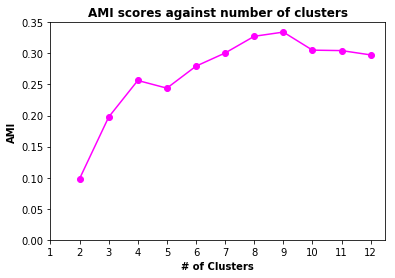
\includegraphics[width=0.9\textwidth]{graphs/24.png}
 \end{center}
}



\end{subquestion}

\begin{subquestion}{\label{Q_CLUSTER_TRENDS}(3 points) Discuss any trends and interesting aspects which emerge from the plot. Does this follow from your expectations?}



\answerbox{10em}{
AMI is low for a small number of clusters and increases rapidly. However, score drops for 5 clusters but keeps increasing until 9 clusters, with a score of 0.334. This means that the clustering achieves the best performance. But as we keep increase further the number of clusters, AMI decreases slowly because we reach a point where the centroids start to overlap and datapoints are assigned to themselves. I was expecting to have a low AMI with a small number of clusters and a point where AMI reaches the maximum score and starts decreasing after that peak.
}



\end{subquestion}

\begin{subquestion}{\label{Q_CLUSTER_FOUR}(6 points) Let us investigate the case with four (4) clusters in some more detail. Using seaborn's \href{https://seaborn.pydata.org/generated/seaborn.countplot.html}{\texttt{countplot}} function, plot a bar-chart of the number of data-points with a particular class (encoded by colour) assigned to each cluster centre (encoded by position on the plot's x-axis). As part of the cluster labels, include the total number of data-points assigned to that cluster.}



\answerbox{40em}{
\begin{center}
 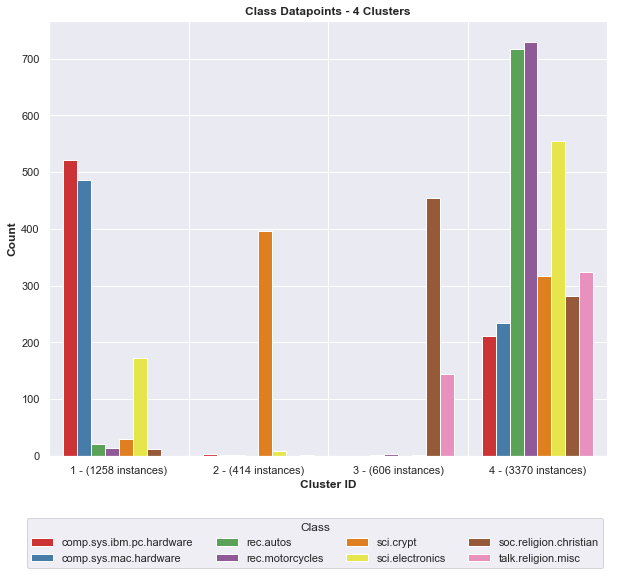
\includegraphics[width=0.9\textwidth]{graphs/26.png}
 \end{center}
}



\end{subquestion}

\begin{subquestion}{(3 points) How does the clustering in Question\ref{Q_UNSUP_LEARN}:\ref{Q_CLUSTER_FOUR} align with the true class labels? Does it conform to your observations in Question\ref{Q_UNSUP_LEARN}:\ref{Q_CLUSTER_TRENDS}?}



\answerbox{14em}{
The clustering and the true labels do not align very well with their true classes. Both the red and blue bars belong to the bigger class 'comp', and we observe that both of these are grouped together in cluster 1. As for cluster 2, we observe that it clearly aligns with 'sci.crypt' class. Regarding cluster 3, most of the datapoints belong to 'soc.religion.christian' class. In cluster 4, although the 'rec' classes dominate the cluster, we see that quite a lot of datapoints of class 'sci.electronics' are assigned to this cluster. So, we observe that most of the instances are assigned to clusters with their corresponding headers (comp, sci, rec...) but are not aligned with their actual correct classes. This is reflected in our 2.5 graph, where the AMI score for 4 clusters is higher than for 5.
}



\end{subquestion}



\end{question}

%============================================================================%

\begin{question}{(26 points) Logistic Regression Classification}
\label{Q_LR_NG}
\questiontext{We will now try out supervised classification on this data. We will focus on Logistic Regression and measure performance in terms of the \href{https://scikit-learn.org/stable/modules/generated/sklearn.metrics.f1_score.html}{F1} score (familiarise yourself with this score which is related to the precision and recall scores that we learnt about in class).}



\begin{subquestion}{(3 points) What is the F1-score, and why is it preferable to accuracy in our problem? How does the macro-average work to extend the score to multi-class classification?}



\answerbox{8em}{
F1-score is a weighted average of precision and recall. In our problem, accuracy can be harmful because we might never classify any instances to class 7, but the model should try to minimise these FNs. F1-score measures misclassified instances better than accuracy and penalises extreme values. The macro-average computes F1-score independently for each class and then takes the average, treating all classes equally without considering imbalanced classes, which can result in a misleading F1-score.
}



\end{subquestion}


\begin{subquestion}{(2 points) As always we start with a simple baseline classifier. Define such a classifier (indicating why you chose it) and report its performance on the \textbf{Test} set. Use the `macro' average for the \texttt{f1\_score}.} %\hint{For the baseline, the classifier should use only the target labels.}



\answerbox{8em}{
I chose a classifier that classifies all instances to the most probable class, which is the class most of the instances in the training dataset are classified to, as my baseline. This seems like a reasonable classifier because if we classify all instances to the most common class (class with most observations), we will make less misclassifications. As we can observe from the F1-score obtained (0.0292), the performance of this classifier on the test set is really bad.
}



\end{subquestion}

\begin{subquestion}{(3 points) We will now train a \href{https://scikit-learn.org/stable/modules/generated/sklearn.linear_model.LogisticRegression.html}{LogisticRegression} Classifier from SKLearn. By referring to the documentation, explain how the Logistic Regression model can be applied to classify multi-class labels as in our case. \hint{Limit your explanation to methods we discussed in the lectures.}}



\answerbox{9em}{
Muticlass classification can be achieved with Logistic Regression by using the one-vs-rest classification, which is a better approach than softmax or sigmoid, for multiclass. In OvR, a Logistic Regression classifier is trained for each class c in our dataset to predict the probability that y=c. So it turns out to be a binary classification where we have a separate binary classifier for each class c, and we calculate whether the datapoing belongs to that class or not.
}



\end{subquestion}

\begin{subquestion}{(4 points) Train a Logistic Regressor on the training data. Set \texttt{solver=`lbfgs'}, \texttt{multi\_class=`multinomial'} and \texttt{random\_state=0}. Use the Cross-Validation object you created and report the average validation-set F1-score as well as the standard deviation. Comment on the result.}



\answerbox{9em}{
Mean F1-score is 0.66899 and standard deviation is 0.01692. Given the average F1-score obtained is 0.67, we can say that the performance of the regressor is quite good and above average 0.5. We also observe that most of the F1-scores obtained are quite low, which indicates that they are not very spread out and are close to the mean (reflected on the low standard deviation).
}



\end{subquestion}

\begin{subquestion}{\label{Q_LOG_REG_PLT}(5 points) We will now optimise the Regularisation parameter $C$ using cross-validation. Train a logistic regressor for different values of $C$: in each case, evaluate the F1 score on the training and validation portion of the fold. That is, for each value of $C$ you must provide the training set and validation-set scores per fold and then compute (and store) the average of both over all folds. Finally plot the (average) training and validation-set scores as a function of $C$. \hint{Use a logarithmic scale for $C$, spanning 19 samples between $10^{-4}$ to $10^5$.}}



\answerbox{40em}{
\begin{center}
 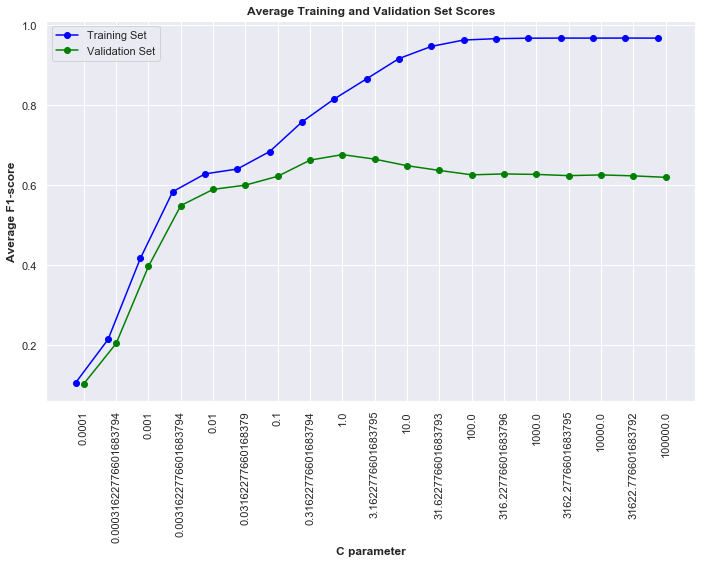
\includegraphics[width=1\textwidth]{graphs/35.png}
 \end{center}
}



\end{subquestion}

\begin{subquestion}{(7 points) What is the optimal value of $C$ (and the corresponding score)? How did you choose this value? By making reference to the effect of the regularisation parameter $C$ on the optimisation, explain what is happening in your plot from Question \ref{Q_LR_NG}:\ref{Q_LOG_REG_PLT} \hint{Refer to the documentation for $C$ in the \href{https://scikit-learn.org/stable/modules/generated/sklearn.linear_model.LogisticRegression.html}{LogisticRegression} page on SKLearn}.}



\answerbox{11em}{
C=1.0 because we obtain the highest average F1-score (0.6768), which means that our regressor generalises the best for C=1.0 on the validation set. The smaller the value of parameter C, the stronger the regularisation and the larger the value, the weaker the regularisation. We regularise to reduce the generalisation error, and not the training error; and to reduce overfitting of the model to the training dataset. So, although we obtain higher F1-scores for higher C values, our model overfits to the training dataset and does not generalise well on unseen data. Thus, the optimal value is for the C that has the highest score.
}



\end{subquestion}

\begin{subquestion}{(2 points) Finally, report the score of the best model on the test-set, after retraining on the entire training set (that is drop the folds). \hint{You may need to set \texttt{max\_iter = 200}.} Comment briefly on the result.}



\answerbox{7em}{
The F1-score obtained on the actual test set is 0.6748. This is expected given that the value we obtained on the validation set for C=1.0 during our cross validation was approximately 0.6768. So, the value we get when we train our model on the testing set reflects our F1-score obtained during our cross validation on the validation set.
}



\end{subquestion}


\end{question}




%============================================================================%




%%%%%%%%%%%%%%%%%%%%%%%%%%%%%%%%%%%%%%%%%%%%%%%%%%%%%%%%%%%%%%%%%%%%%%%%%%%%%%
%============================================================================%
%%%%%%%%%%%%%%%%%%%%%%%%%%%%%%%%%%%%%%%%%%%%%%%%%%%%%%%%%%%%%%%%%%%%%%%%%%%%%%

\clearpage

\assignmentSection{Part B: Bristol Air-Quality [90 points]}




\begin{question}{\label{Q_EXPLORATORY}(30 Points) Exploratory Analysis}

\questiontext{We will begin by exploring the Dataset to familiarise ourselves with it.}



\begin{subquestion}{(6 points) Summarise the key features/observations in the data: describe the purpose of each column and report (briefly) also on the dimensionality/ranges (ballpark figures only, and how they compare across features) and number of sites, and identify anything out of the ordinary/problematic: \ie look out for missing data and negative values. Why are the latter unreasonable in such a dataset? \hint{Refer to the documentation for how to interpret the pollutant values.}}



\answerbox{13em}{
1,306,758 instances and 7 attributes. 'Date Time' (object) states the date and time that of the reading. The values range from '1993-01-01' to '2019-08-12'. NOx, NO2, NO (float), refer to the amount of these chemicals, and are the most problematic given that some entries have missing data and others have negative values (ug/m3 cannot be negative). They range between -31.08 to 2164.25, -6.6698 to 576.5 and -17.71 to 1231.24 respectively. 576 readings are negative and 118872 have missing data (NaN). These problematic values are unreasonable since the dataset focuses mainly on air pollution. SiteID (integer), uniquely identifies air pollution entries from same location (18 unique locations). Loc.Lat and Loc.Long (float) define the coordinates and range between 51.43 and 51.49, and -2.69 and -2.54 respectively.
}



\end{subquestion}

\begin{subquestion}{(6 points) Repeat the same analysis but this time on a per-site basis. Provide a table with the number of samples and percentage of problematic samples (negative and missing) in each site. To report numbers, count a row which has at least one missing entry
as having missing data, and similarly for negative entries. \hint{Pandas has a handy method, \texttt{to\_latex()}, for generating a latex table from a dataframe.}}



\answerbox{17em}{
\begin{tabular}{rrrrrrrr}
\toprule
 Site &  Samples &  Missing\% &  Negative\% &  Site &  Samples &  Missing\% &  Negative\% \\
\midrule
       0 &     6446 &      1.613 &        0.00 &        9 &    22071 &      5.301 &        0.00 \\
       1 &   163111 &      6.290 &        0.00 &       10 &    96407 &      3.590 &        0.00 \\
       2 &    62990 &      4.348 &        0.00 &       11 &    20693 &      1.904 &        0.09 \\
       3 &    25464 &     77.333 &        0.78 &       12 &    45240 &     17.485 &        0.00 \\
       4 &    74787 &      2.069 &        0.01 &       13 &    12423 &     51.461 &        0.02 \\
       5 &   113952 &      8.828 &        0.00 &       14 &   113951 &     10.532 &        0.00 \\
       6 &   142141 &      7.444 &        0.00 &       15 &     2712 &    100.000 &        0.00 \\
       7 &   115162 &      4.195 &        0.28 &       16 &   154331 &      6.531 &        0.01 \\
       8 &    43824 &     21.057 &        0.00 &       17 &    91053 &      6.271 &        0.00 \\
\bottomrule
\end{tabular}
}



\end{subquestion}

\begin{subquestion}{(4 points) Briefly summarise how the sites compare in terms of number of samples and amount of problematic samples.}



\answerbox{11em}{
118,872 instances out of 1,306,758 in our initial dataset, have at least one missing value. All 18 sites have at least one missing data in the gas readings. All entries for Site 15 have missing values and Site 3 has 77.33\% missing values out of the total 25,464 Site 3 instances. Site 0 has the lowest relative amount of missing values. 576 entries in the dataset have negative values, relatively less than missing data. Not all sites have negative readings. Only sites 3, 7, 13 and 16 have negative valued data. Site 3 has the highest percentage of negative valued data. But overall, there are not many negative values. So, Site 3 has a high percentage of problematic data.
}



\end{subquestion}

\begin{subquestion}{(3 points) Given that the columns are all oxides of nitrogen and hence we expect them to be related, we will now look at correlations in our data. This will also be useful in determining how well we can predict any one of the readings from the other two. Remove the data from sites 3 and 15 and compute the \textbf{Pearson} correlation coefficient between each of the three pollutant columns on the remaining data. Visualise the coefficients between each pair of columns in a table.}



\answerbox{10em}{
\begin{tabular}{lrrr}
\toprule
{} &    NOx &    NO2 &     NO \\
\midrule
NOx &  1.000 &  0.878 &  0.988 \\
NO2 &  0.878 &  1.000 &  0.808 \\
NO  &  0.988 &  0.808 &  1.000 \\
\bottomrule
\end{tabular}
}



\end{subquestion}

\begin{subquestion}{(2 points) Comment on the level of correlation between each pair of pollutants.}



\answerbox{7em}{
As expected, all diagonal values are very strongly correlated, with maximum correlation of 1, because they are paired with themselves. The most correlated pair is NO and NOx, with a correlation coefficient of 0.99, followed by the pair NO and NO2, and lastly NO2 and NOx which are the least correlated pair out of the three possible pairs with a value of 0.88.
}



\end{subquestion}



\begin{subquestion}{\label{CORRELATIONS}(5 points) For each of the three pollutants, compute the Pearson correlation between sites. \hint{You will need to remove the `Date Time' column and then group by the first level of the columns.} Then plot these as three heatmaps: show the values within the figures. \hint{Use the method \texttt{plot\_matrix()} from \texttt{mpctools.extensions.mplext}.}}



\answerbox{40em}{
\begin{center}
 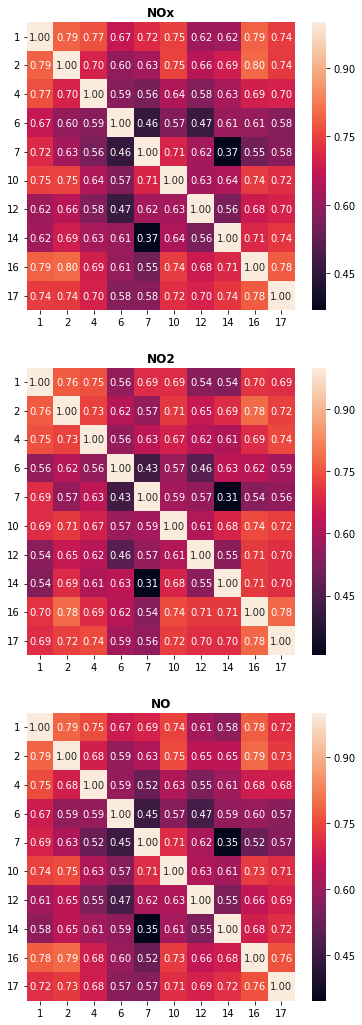
\includegraphics[width=0.38\textwidth]{graphs/46.png}
 \end{center}
}



\end{subquestion}

\begin{subquestion}{(4 points) Comment briefly on your observations from Question \ref{Q_EXPLORATORY}:\ref{CORRELATIONS}: start by summarising the results from the NO gas and then comment on whether the same is observed in the other gases or if there is something different.}



\answerbox{12em}{
In the NO gas heatmap, the highest correlated sites are the pairs (1,2) and (2,16), both with correlation coefficient 0.79, which means that these location pairs' pollution quantity is similar. Regarding the NO2 gas, we observe that indeed (2,16) are the highest correlated location pair, followed by (1,2).  And for NOx gas, (2,16) is the highest correlated pair followed by (1,2) and (1,16). Thus, we can conclude that the nitrogen oxides of locations 2 and 16 are the most related out of all the sites. The least correlated pair, in the NO heatmap the pair (7,14) has the lowest correlation, and as expected, the same location pair has the lowest value for the three gases. So, we can say that the locations 7 and 14 have the least related gases.
}



\end{subquestion}

\end{question}


%============================================================================%

\begin{question}{(19 Points) Principal Component Analysis}

\questiontext{One aspect which we have not yet explored is the temporal nature of the data. That is, we need to keep in mind that the readings have a temporal aspect to them which can provide some interesting insight. We will explore this next.}



\begin{subquestion}{(1 point) Plot the first 5 lines of data (plot each row as a single line-plot).}



\answerbox{40em}{
\begin{center}
 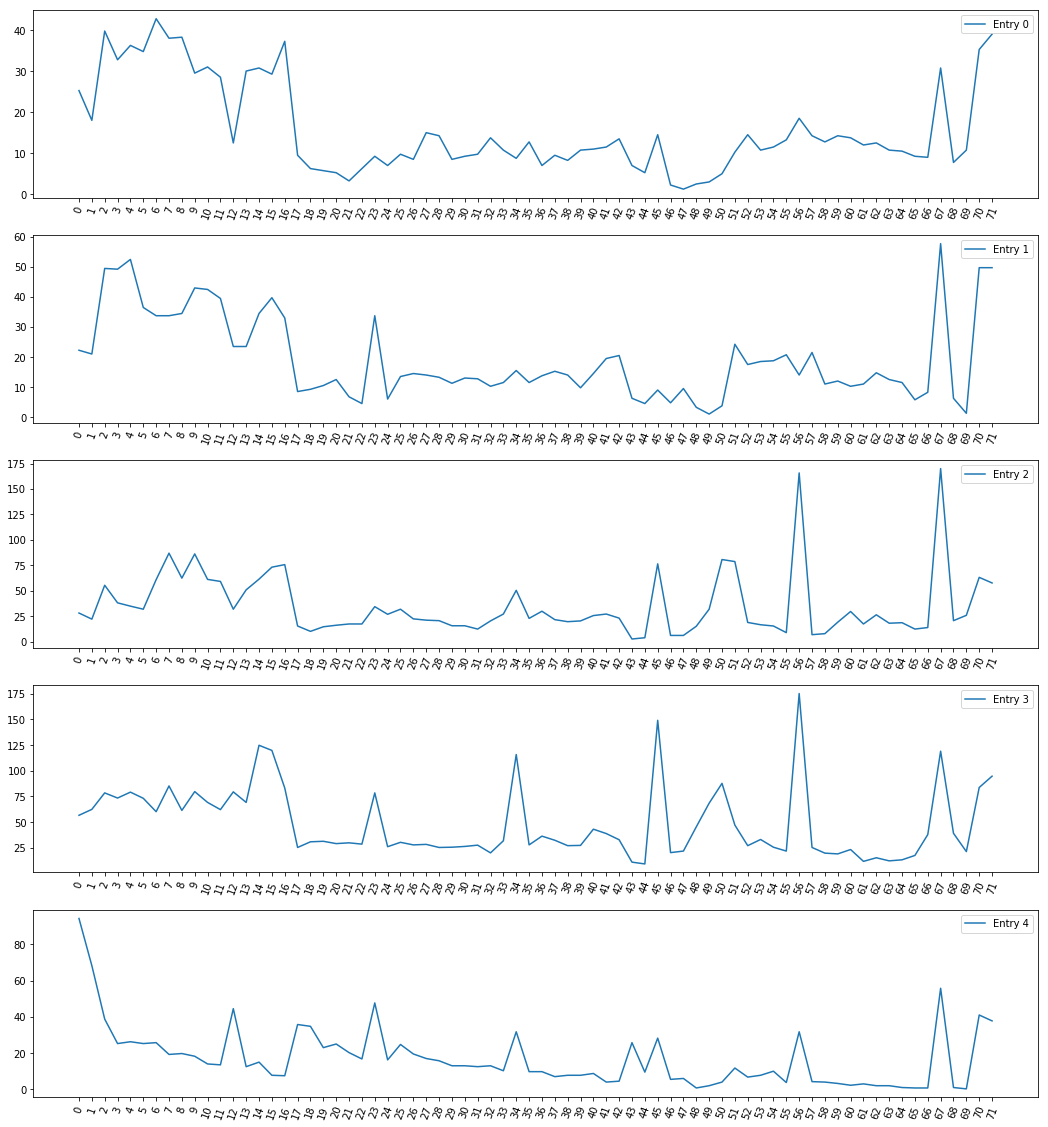
\includegraphics[width=0.98\textwidth]{graphs/51.png}
 \end{center}
}



\end{subquestion}



\begin{subquestion}{(5 points) We will focus first on data solely from Site 1. Extract the data from this site, and run PCA with the number of components set to 72 for now. Set the \texttt{random\_state=0}. On a single graph plot: (i) the percentage of the variance explained by each principal component (as a bar-chart), (ii) the cumulative variance (line-plot) explained by the first $n$ components: (\hint{you should use \href{https://matplotlib.org/3.1.1/api/_as_gen/matplotlib.axes.Axes.twinx.html}{\texttt{twinx()}} to make the plot fit}), \textsl{and}, (iii) mark the point at which the number of components collectively explain at least 95\% of the variance (using a vertical line). \hint{Number components starting from 1.}}



\answerbox{40em}{
\begin{center}
 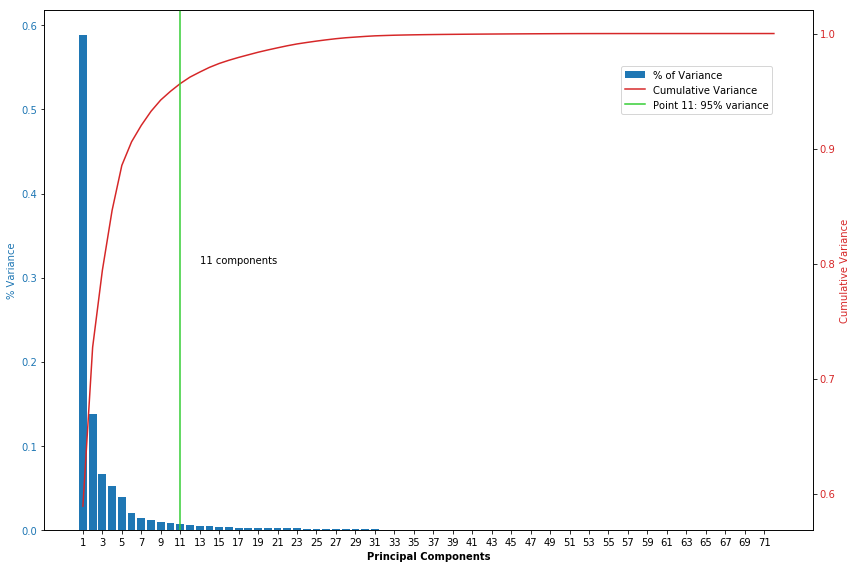
\includegraphics[width=1\textwidth]{graphs/52.png}
 \end{center}
}



\end{subquestion}

\begin{subquestion}{(2 points) Interpret and summarise the above plot.}



\answerbox{9em}{
PC1 accounts for as much of the variability, and each of the succeeding components account for as much of the remaining variability as possible. As expected, PC1 has the highest variance (59\%), and the variance explained by each PC decreases as we increase the number of principal components. (PC2 has variance 14\%). The first 11 components account for just over 95\% of the variance, so we cover for most of the important features in our original dataset with 11 PCs.
}



\end{subquestion}


\begin{subquestion}{(5 points) Generate three figures, one for the mean and one for each of the first 2 principal components: in each, plot the mean/component as three lines, one for each pollutant throught one day cycle. \hint{You will need to reshape the components appropriately.}}



\answerbox{50em}{
\begin{center}
 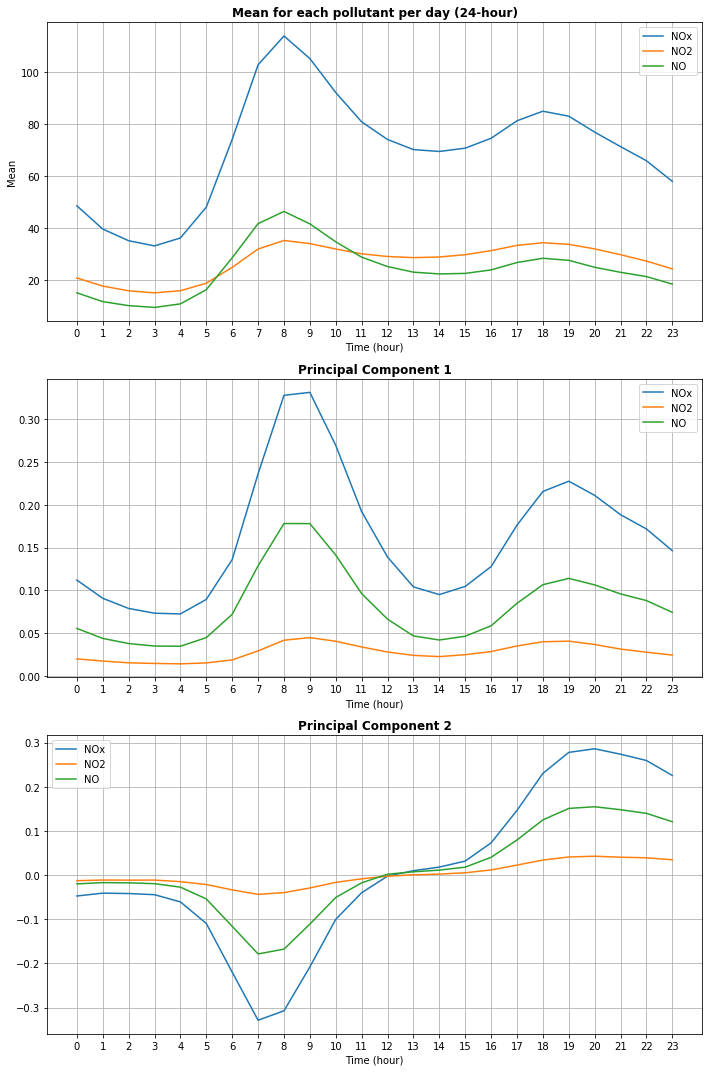
\includegraphics[width=0.9\textwidth]{graphs/54.png}
 \end{center}
}



\end{subquestion}

\begin{subquestion}{(6 points) Focusing on the mean and first principal component, are there any significant patterns which emerge throughout the day? \hint{Think about car usage throughout the day.} What is different when interpreting the mean versus the first component? \hint{Do peaks signify the same thing in both cases?} Looking at the principal components only, are there any significant differences between the pollutants? Why could this be happening? \hint{You can refer to one of the limitations of PCA.}}



\answerbox{16em}{
PC1 follows the pattern of the mean but with no overlaps between any pollutants. Around 8-9am and 6-7pm, the 3 gases peak, because of rush hour times (car usage). Difference between mean and PC1 is that mean denotes the average readings for each pollutant whereas PC1 is the direction in space along which, projections have the largest variance. Our graph denotes the projections of each data instance onto our vector for PC1.  As expected, variance is high, so the data is spread out (no overlaps in PC1). Comparing the two PCs, PC2 is the direction that maximises variance among all directions, and is perpendicular to PC1. In the PC2 graph we get negative values between 0-12pm, which means that the projections' directions is opposite to the direction of the PC, i.e., a negative relationship, so a high value. PCA relies on linear assumptions and looks for orthogonal projections that contain highest variance possible, to find a hidden linear correlation between the attributes.
}



\end{subquestion}

\end{question}

%============================================================================%


\begin{question}{\label{Q_LR_BA}(41 points) Regression}


\questiontext{Given our understanding of the correlation between signals and sites, we will now attempt to predict the NOx level for Site 17 given the value at the other sites. We will evaluate our models using the Root Mean Squared Error (RMSE) \ie the square root of the \href{https://scikit-learn.org/stable/modules/generated/sklearn.metrics.mean_squared_error.html}{mean\_squared\_error} score by sklearn.}



\begin{subquestion}{(2 points) First things first: since we are dealing with a supervised task, we will need to split our data into a training and testing set. Furthermore, since some of our regressors will involve hyper-parameter tuning, we will also need a validation set. Use the \texttt{multi\_way\_split()} method from \texttt{mpctools.extensions.skext} to split the data into a Training (60\%), Validation (15\%) and Testing (25\%) set: use the \href{https://scikit-learn.org/stable/modules/generated/sklearn.model_selection.ShuffleSplit.html}{ShuffleSplit} object from sklearn for the \texttt{splitter}. Set the random state to 0. \hint{The method gives you the indices of the split for each set, which can then be applied to multiple matrices.} Report the sizes of each dataset.}



\answerbox{4em}{
Training set has 8937 instances, validation set has 2234 instances and testing set has 3724 instances.
}



\end{subquestion}

\begin{subquestion}{(4 points) Let us start with a baseline. By using only the $y$-values, what baseline regressor can you define (indicate what it does)? Implement it and report the RMSE on the training and validation sets. Interpret this relative to the statistics of the data.}



\answerbox{8em}{
Baseline always predicts average of the target. RMSE for training set is 79.71 and 80.21 for validation. Given that our baseline predicts the mean, MSE turns out to be variance; and RMSE the standard deviation. The maximum target value in training is 801.25 and 656.5 in validation, and the minimum is 0.75 for both. Model prediction is 98.32, which is quite far from most of the actual predictions, thus the high error scores.
}



\end{subquestion}

\begin{subquestion}{(3 points) Let us now try a more interesting algorithm: specifically, we will start with \href{https://scikit-learn.org/stable/modules/generated/sklearn.linear_model.LinearRegression.html}{LinearRegression}. Train the regressor on the training data and report the RMSE on the training and validation set, and comment on the relative performance to the baseline.}



\answerbox{7em}{
We observe that the error is relatively lower than for the baseline regressor, which means our model is more accurate and the predictions are closer to the line of best fit. Moreover, the RMSE on the validation set is not much higher than that on the training set, so we could say our model does not overfit to the training data (although further analysis and inspection would be needed to conclude this).
}



\end{subquestion}



\begin{subquestion}{(5 points) We want to explore further what the model is learning. Explain why in Linear Regression, we cannot just blindly use the weights of the regression coefficients to evaluate the relative importance of each feature, but rather we have to normalise the features. By referring to the documentation for the \href{http://scikit-learn.org/stable/modules/generated/sklearn.linear_model.LinearRegression.html}{LinearRegression} implementation in SKLearn, explain what the normalisation does and how it helps in comparing features. Will this affect the performance of the Linear Regressor?}



\answerbox{10em}{
Normalising is important to make different models comparable. This way, values will range over a common scale. This way, the actual true information in a feature can be captured and we avoid giving more importance to features who have higher ranges. If we did not normalise, this use of weights would not be accurate. We would be overweighing those particular features with larger values, and make our model predictions biased towards these features with high values. Thus, normalising affects the magnitude of the coefficients but does not affect performance of the regressor.
}



\end{subquestion}

\begin{subquestion}{(5 points) Retrain the regressor, setting \texttt{normalize=True} and report (in a table) the ratio of the relative importance of each feature. Which is the most/least important site? How do they compare with the correlation coefficients for Site 17 as computed in Question \ref{Q_EXPLORATORY}:\ref{CORRELATIONS}, and why do you think that is?}



\answerbox{15em}{
Site 16 is the most important site, with a relative importance of 0.16, whereas the least important is Site 6 with a value of -0.0068 and is negatively correlated. By comparing these values with the correlation coefficients for Site 17 obtained in 4.6, we observe that the site that has the highest correlation coefficient with Site 17 is indeed Site 16 for all three pollutants, and Site 6 is not very correlated with Site 17. So, we can deduce that highly correlated sites have a high relative importance value too. But this is not necessarily always true. Site 2 has a low importance value of 0.0099, but is highly correlated with Site 17.
}



\end{subquestion}

\begin{subquestion}{(5 points) It might be that with non-linear models, we may get better performance. Let us try to use \href{https://scikit-learn.org/stable/modules/generated/sklearn.neighbors.KNeighborsRegressor.html}{K-Nearest-Neighbours}. Train a KNN regressor with default parameters on the training set and report performance on the training and validation set. \hint{it might be beneficial to set \texttt{n\_jobs=-1} to improve performance.} How does it compare with Linear Regression in terms of performance on both sets? What is a limitation of the KNN algorithm for our dataset?}



\answerbox{8em}{
RMSE on training is 39.835 and 41.127 on validation. Linear performs better on validation set, relative to its training set; whereas the kNN regressor has a much lower error on training set, but does not perform that well on validation; so it does not generalise well. Limitation of kNN is that it does not work well on large datasets(14895)/dimensions(16) because it computes the distance for each datapoint at each iteration, for each dimension. so it has a high computational cost.
}



\end{subquestion}

\begin{subquestion}{(4 points) The KNN regression allows setting a number of hyper-parameters. We will optimise only one: the number of neighbours to use. By using the validation set, find the optimal value for the \texttt{n\_neighbours} parameter out of the values [2, 4, 8, 16, 32]. Plot the training/validation RMSE and indicate (for example with a line) the best value for \texttt{n\_neighbours}.}



\answerbox{40em}{
\begin{center}
 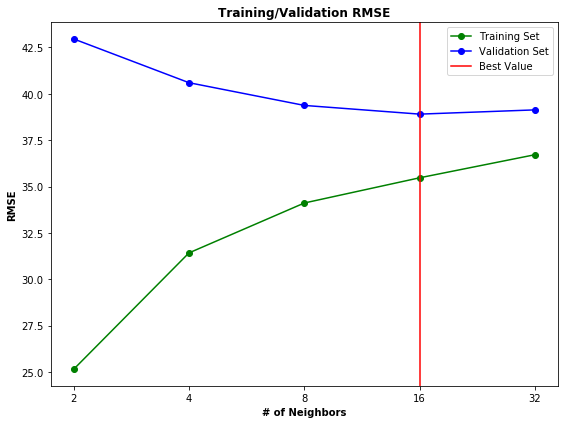
\includegraphics[width=1\textwidth]{graphs/68.png}
 \end{center}
}



\end{subquestion}

\begin{subquestion}{(1 points) What is the best-case RMSE performance on the validation set for KNN?}



\answerbox{6em}{
Best value for n\_neighbors on the validation set is 16 neighbours, which has lowest RMSE value of 38.9018 on validation set. This is because the lower the error the better our model generalises on unseen data.
}



\end{subquestion}

\begin{subquestion}{(4 points) Let us try one last regression algorithm: we will now use \href{https://scikit-learn.org/stable/modules/generated/sklearn.tree.DecisionTreeRegressor.html}{DecisionTreeRegressor}. Again, the algorithm contains a number of hyper-parameters, and we will optimise the depth of the tree. Train a series of Decision Tree Regressors, optimising (over the validation set) the \texttt{max\_depth} over the values [2, 4, 8, 16, 32, 64]. Set \texttt{random\_state=0}. Plot the training/validation RMSE and indicate (as before) the best value for \texttt{max\_depth}.}



\answerbox{40em}{
\begin{center}
 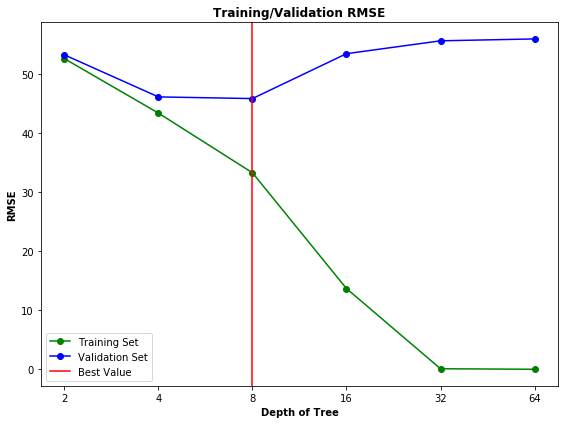
\includegraphics[width=1\textwidth]{graphs/69.png}
 \end{center}
}



\end{subquestion}

\begin{subquestion}{(3 points) What is the best-case RMSE performance on the validation set? What do you notice from the plot about the performance of the Decision Tree Regressor?}



\answerbox{6em}{
Best case obtained for depth 8, with RMSE 45.8438. However, the regressor is overfitting. As we increase the depth, error decreases significantly on training set and becomes 0 at depth 32. But for validation set, error keeps increasing. So, the DT does not generalise well on unseen data.
}



\end{subquestion}

\begin{subquestion}{(5 points) To conclude let us now compare all the models on the testing set. Combine the training and validation sets and retrain the model from each family on it: in cases where we optimised hyper-parameters, set this to the best-case value. Report the testing-set performance of each model in a table \hint{You should have 4 values}.}



\answerbox{6em}{
\begin{tabular}{lllll}
\toprule
{} & Baseline &  Linear & Nearest Neighbours & Decision Tree \\
\midrule
RMSE &  78.952 &  40.509 &             37.985 &       43.069 \\
\bottomrule
\end{tabular}
}



\end{subquestion}

\end{question}

%============================================================================


\end{document}
